%% Supersede --- CEUR-ART single-column paper.
\documentclass[]{ceurart}

\sloppy

\usepackage{listings}
\lstset{breaklines=true}
\usepackage{tikz}
\usetikzlibrary{arrows.meta, positioning, fit, backgrounds}
\usepackage{amsmath}

\begin{document}

\copyrightyear{2026}
\copyrightclause{Copyright for this paper by its authors.
  Use permitted under Creative Commons License Attribution 4.0
  International (CC BY 4.0).}

\conference{Preprint, 2026}

\title{Supersede: Diagnosing and Training Memory-Consistent Agents under Fact Supersession}

\author[1]{Vedant Patel}[%
email=vedant@vrin.cloud,
url=https://vrin.cloud,
]
\cormark[1]
\address[1]{Vrin (Independent Researcher), United States}

\cortext[1]{Corresponding author.}

\begin{abstract}
  Large language model (LLM) agents increasingly operate over long,
  multi-session interactions in which facts change: a user moves, a price
  updates, a plan is revised. Acting correctly requires using the
  \emph{current} value of a fact and discarding values that have been
  \emph{superseded}. We isolate this ability on real conversational data and
  show that it is a distinct, unsolved failure. On the
  \texttt{knowledge-update} subset of LongMemEval, replacing an agent's full
  context with a bounded, self-maintained memory drops accuracy from
  $92\%$ to $77\%$ even on a frontier model (gpt-5.4), a gap that is
  statistically significant (paired McNemar $p<0.005$) and \emph{persists
  across model scale} while full-context accuracy saturates near $92\%$. The
  bottleneck is therefore memory maintenance, not comprehension, and it is not
  closed by a stronger model. We further show that synthetic, templated
  supersession is saturated ($100\%$) and thus fails to surface the problem,
  explaining why it is under-measured. Finally, we release \textbf{Supersede},
  an open reinforcement-learning environment (built on the \texttt{verifiers}
  /\,\texttt{prime-rl} stack) that turns this measurement into a training
  signal: agents are rewarded for answering from the current value and
  penalized for stale ones. The environment reproduces the failure
  end-to-end and is, to our knowledge, the first trainable environment whose
  reward targets temporal fact-currency.
\end{abstract}

\begin{keywords}
  LLM agents \sep
  long-term memory \sep
  knowledge updates \sep
  reinforcement learning environments \sep
  evaluation
\end{keywords}

\maketitle

\section{Introduction}

Pre-training has largely consumed the open web, and the frontier of LLM
capability has shifted toward agents that act over long horizons using
\emph{external memory} rather than a single context window. A defining
property of long-horizon interaction is that information is not static: facts
are introduced, then later updated or retracted. An assistant that is told a
user lives in Detroit, and later that they moved to the suburbs, must answer a
subsequent location question with the \emph{current} value. We call the
correct handling of such updates \emph{supersession}.

Recent benchmarks have begun to measure long-term memory
\cite{maharana2024locomo, wu2025longmemeval, memoryarena2026,
memoryagentbench2025, fama2026}, and a forgetting-aware metric has been
proposed to penalize reliance on obsolete information \cite{fama2026}. These
works, however, score \emph{frozen} models: they quantify the problem but do
not provide a mechanism to \emph{train} it away. In parallel, a line of work
applies reinforcement learning to memory agents \cite{memagent2025,
longrlvr2026}, but rewards final-answer correctness or evidence relevance,
never temporal currency. No existing work sits in the intersection: a
\emph{trainable} environment whose reward is supersession-correctness.

This paper makes three contributions.

\begin{enumerate}
  \item \textbf{An isolation result.} On real conversational data, we hold
  memory load fixed and vary only whether the agent has full context or a
  bounded, self-maintained memory. Bounded memory degrades
  \texttt{knowledge-update} accuracy significantly (Section~\ref{sec:results}),
  isolating memory maintenance --- not reading comprehension --- as the cause.
  \item \textbf{A frontier, scale-robust confirmation.} The gap survives on
  gpt-5.4 ($92\%\!\rightarrow\!77\%$, $p=0.0033$) and does not shrink to zero
  as the model improves; full-context accuracy, by contrast, saturates. A
  negative control shows synthetic templated supersession is saturated and
  therefore uninformative.
  \item \textbf{An open environment.} We release \textbf{Supersede}, a
  \texttt{verifiers}/\texttt{prime-rl} environment with a programmatic
  supersession-aware reward, validated end-to-end. It reframes the
  forgetting-aware \emph{metric} of \cite{fama2026} as a \emph{learning
  signal}.
\end{enumerate}

\section{Related Work}

\paragraph{Long-term memory benchmarks.} LoCoMo \cite{maharana2024locomo}
evaluates very long multi-session dialogue but does not annotate a dedicated
update category. LongMemEval \cite{wu2025longmemeval} introduces an explicit
\texttt{knowledge-update} question type in which a fact stated in one session
is changed in a later one; we adopt this subset as ground truth. MemoryArena
\cite{memoryarena2026} shows that models near-perfect on recall benchmarks
drop sharply when memory must drive actions, motivating evaluation beyond
passive recall. MemoryAgentBench \cite{memoryagentbench2025} includes a
conflict-resolution competency. Memora and its FAMA metric \cite{fama2026}
explicitly penalize reliance on superseded or deleted memory. All of these are
evaluation-only.

\paragraph{Memory systems and RL for memory.} Mem0 \cite{chhikara2025mem0}
manages a memory store with prompted \textsc{add}/\textsc{update}/\textsc{delete}
operations --- a heuristic, not a learned, policy. MemAgent
\cite{memagent2025} trains a memory agent with RL but rewards only
final-answer correctness; LongRLVR \cite{longrlvr2026} adds a verifiable
reward on evidence \emph{relevance} within a single long document. Neither
rewards \emph{temporal currency} across sessions. Supersede generalizes the
verifiable-reward idea of \cite{longrlvr2026} to a time-indexed signal and
operationalizes the FAMA metric of \cite{fama2026} as a reward.

\paragraph{Environment infrastructure.} We build on the \texttt{verifiers}
library and the Prime Intellect Environments Hub
\cite{primeintellect2025environments}, which standardize environments for
post-training, and are compatible with the emerging OpenEnv standard
\cite{openenv2025}.

\section{The Supersede Environment}
\label{sec:env}

\paragraph{Task.} A task is a multi-session interaction followed by a query
about the current value of a fact that changed during the interaction. The
agent processes one session at a time and maintains a \emph{bounded} memory
(a notes field capped at $B$ characters); crucially, raw sessions are
\emph{never re-fed}. After the final session, the agent answers the query using
its memory alone. Figure~\ref{fig:rollout} shows the rollout.

\begin{figure}[t]
  \centering
  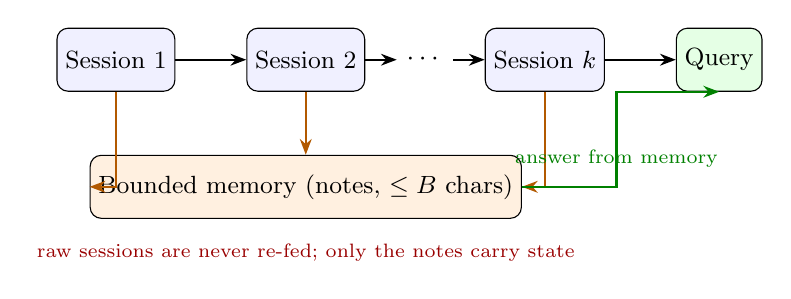
\begin{tikzpicture}[
    node distance=6mm and 9mm,
    box/.style={draw, rounded corners, align=center, font=\small,
                minimum height=8mm, inner sep=3pt},
    sess/.style={box, fill=blue!6},
    mem/.style={box, fill=orange!12},
    q/.style={box, fill=green!10},
    arr/.style={-{Stealth[length=2mm]}, thick},
  ]
    \node[sess] (s1) {Session 1};
    \node[sess, right=of s1] (s2) {Session 2};
    \node[right=4mm of s2] (dots) {$\cdots$};
    \node[sess, right=4mm of dots] (sk) {Session $k$};
    \node[q, right=of sk] (qq) {Query};

    \node[mem, below=8mm of s2] (m) {Bounded memory (notes, $\le B$ chars)};

    \draw[arr] (s1) -- (s2);
    \draw[arr] (s2) -- (dots);
    \draw[arr] (dots) -- (sk);
    \draw[arr] (sk) -- (qq);

    \draw[arr, orange!70!black] (s1) |- (m.west);
    \draw[arr, orange!70!black] (s2) -- (m);
    \draw[arr, orange!70!black] (sk) |- (m.east);
    \draw[arr, green!50!black] (m.east) -- ++(1.2,0) |- (qq.south)
      node[pos=0.25, below, font=\scriptsize] {answer from memory};

    \node[font=\scriptsize, text=red!60!black, below=2mm of m]
      {raw sessions are never re-fed; only the notes carry state};
  \end{tikzpicture}
  \caption{The Supersede rollout. The agent rewrites a bounded notes memory
  after each session and answers the final query from memory alone. Because
  history is not re-fed, a superseded value that is not overwritten persists
  and corrupts the answer.}
  \label{fig:rollout}
\end{figure}

\paragraph{Reward.} The primary reward is $r_{\text{cur}}=\mathbb{1}[\text{the
final answer conveys the current value}]$, scored by a programmatic,
ungameable matcher (normalized variant match with a token-overlap fallback),
so the environment can be evaluated and trained without an auxiliary judge
model. When the superseded values are known (our synthetic tasks, or
update-annotated items), a penalty
$r_{\text{stale}}=-\mathbb{1}[\text{the answer asserts a superseded value}]$
is added; on gold-only data it is inert. The combined reward is
$r = r_{\text{cur}} + \lambda\, r_{\text{stale}}$. This makes the
forgetting-aware accuracy of \cite{fama2026} a dense training signal rather
than a post-hoc score.

\paragraph{Data.} Tasks are drawn from the LongMemEval
\texttt{knowledge-update} subset (real conversational supersession) and from a
procedural generator of synthetic timelines used for controls and ablations.
The environment is implemented as a \texttt{verifiers} \texttt{MultiTurnEnv};
the prompt assembly enforces the no-re-feed property, and rollouts terminate
when the answer is produced.

\section{Experimental Setup}

\paragraph{Data and grading.} We use all $78$ \texttt{knowledge-update}
questions from the LongMemEval \emph{oracle} split (evidence sessions only).
Unless noted, answers are graded by an LLM judge following the LongMemEval
protocol; the environment's intrinsic reward uses the programmatic matcher.
\paragraph{Conditions.} \textsc{Full-context} places every evidence session in
the model context and asks the question (an upper bound where memory is not the
bottleneck). \textsc{Bounded-memory} is the Supersede agent of
Section~\ref{sec:env} with $B=300$ characters. \paragraph{Models.} We evaluate
gpt-4.1-mini, gpt-4.1, and the frontier gpt-5.4, at temperature $0$.
\paragraph{Significance.} Because both conditions are run on the same
questions, we use a paired McNemar test.

\section{Results}
\label{sec:results}

\begin{figure}[t]
  \centering
  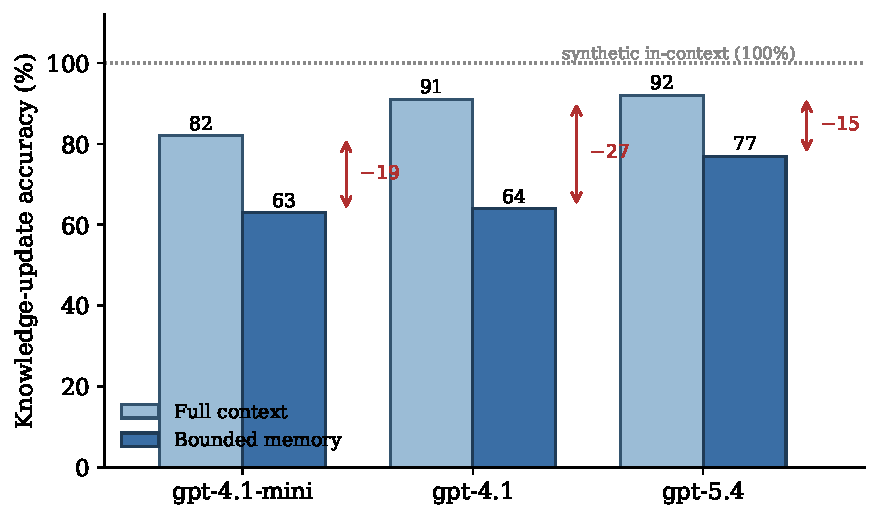
\includegraphics[width=\linewidth]{figures/results.pdf}
  \caption{Knowledge-update accuracy: full context vs.\ bounded memory, across
  three models. Stronger models read context better (full-context rises to
  $92\%$) but bounded-memory accuracy does not catch up; the gap is the cost of
  memory maintenance under updates. The dotted line marks synthetic
  in-context performance ($100\%$), which is saturated and uninformative.}
  \label{fig:results}
\end{figure}

\begin{table}[t]
  \caption{LongMemEval \texttt{knowledge-update} ($n=78$). The
  full-context\,$\rightarrow$\,bounded-memory gap is significant on both the
  small and the frontier model.}
  \label{tab:main}
  \centering
  \begin{tabular}{lccc}
    \toprule
    Model & Full context & Bounded memory & Paired McNemar \\
    \midrule
    gpt-4.1-mini & $82\%$ & $63\%$ & $p=0.0035$ \\
    gpt-4.1      & $91\%$ & $64\%$ & --- \\
    gpt-5.4      & $92\%$ & $77\%$ & $p=0.0033$ \\
    \bottomrule
  \end{tabular}
\end{table}

\paragraph{Bounded memory degrades supersession, significantly.}
Table~\ref{tab:main} and Figure~\ref{fig:results} report the main result. For
gpt-4.1-mini, accuracy falls from $82\%$ to $63\%$; the paired test counts
$19$ questions that full-context answers correctly but bounded-memory does not,
against only $4$ in the reverse direction ($p=0.0035$). Roughly $13\%$ of
questions are wrong even in full context, confirming that real updates are
genuinely hard.

\paragraph{The gap persists on the frontier and does not close with scale.}
gpt-5.4 raises full-context accuracy to $92\%$ but bounded-memory accuracy only
to $77\%$ ($p=0.0033$; $13$ vs.\ $1$). Bounded-memory accuracy across the
family ($63\%, 64\%, 77\%$) improves far more slowly than full-context
accuracy ($82\%, 91\%, 92\%$): scaling the model helps memory maintenance only
partially, while comprehension saturates. The failure is therefore a property
of the memory mechanism, not of model capability.

\paragraph{Failure modes.} Bounded-memory errors are dominated by the relevant
fact being compressed away or not overwritten. Asked ``How many Korean
restaurants have I tried?'' (gold: \emph{four}), the agent answers ``you
haven't mentioned any.'' Asked ``Where did Rachel move to?'' (gold:
\emph{the suburbs}), gpt-5.4 answers ``no information about Rachel.'' In both,
the model is competent but its memory no longer contains the updated fact.

\paragraph{Synthetic supersession is saturated.} As a negative control, we ran
the same models on procedurally generated, templated supersession timelines
(explicit ``$X$ now $Y$'' updates) with full history in context: accuracy is
$100\%$ across configurations. Frontier models trivially resolve clean,
explicit updates by a last-mention scan; the failure only appears with bounded
memory on natural, paraphrased data. This explains why supersession is
under-measured and motivates the use of real data.

\paragraph{Environment validation.} Running the released environment
end-to-end on all $78$ questions, every rollout terminates cleanly and the
intrinsic programmatic reward yields $57.7\%$ for gpt-4.1-mini, consistent with
the $63\%$ measured by the LLM judge (the matcher is stricter). The
environment thus faithfully reproduces the failure it is designed to train
against.

\section{Discussion}

The result reframes supersession from a comprehension problem to a memory-policy
problem. Stronger models read updated context well, but when they must
\emph{decide what to keep} under a bounded budget, they discard or fail to
overwrite the value that later matters. This is precisely the regime that
production memory systems operate in, and precisely where a heuristic
\textsc{update}/\textsc{delete} policy \cite{chhikara2025mem0} is brittle.
Because the gap does not close with scale, waiting for larger models is not a
solution; a memory policy that is \emph{trained} to preserve currency is.
Supersede provides the environment and the verifiable reward to do so.

\section{Limitations}

We report a benchmark-and-environment result, not a trained-policy result:
demonstrating that the reward improves a policy requires RL training and is
left to future work. Grading by LLM judge introduces some noise (a few
bounded-memory failures are judge strictness, e.g.\ ``over 25'' vs.\ gold
``25''); the paired significance survives a handful of such flips. We use the
oracle split; the larger distractor splits should widen the gap and are a
natural next measurement. Finally, the synthetic generator is a control, not a
training target.

\section{Conclusion}

Agents fail at supersession not because they cannot read updates but because
they cannot maintain them under a bounded memory --- a gap that is significant,
reproducible on a trusted benchmark, and unclosed by frontier scale. We release
Supersede, an open environment that turns this forgetting-aware measurement
into a training signal, as a step toward agents whose memory stays current.

\begin{acknowledgments}
  We thank the maintainers of LongMemEval and of the \texttt{verifiers} /
  Prime Intellect Environments Hub for the open datasets and tooling this work
  builds on.
\end{acknowledgments}

\section*{Declaration on Generative AI}
  During the preparation of this work, the author used a code-assistant
  (Claude) for drafting prose, generating figures, and implementing and
  debugging the environment and evaluation code. All experiments, numbers, and
  claims were executed and verified by the author, who reviewed and edited the
  content and takes full responsibility for the publication's content.

\bibliography{refs}

\end{document}
